\section{Теоретические вопросы}
\subsection{Характеристика инвестиционного климата в России. Факторы, определяющие инвестиционный климат}

Высокая инвестиционная активность --- одно из условий развития экономики страны.
Она достигается за счет роста объемов реализуемых инвестиционных ресурсов и их целесообразного использования в различных сферах.
Инвестиции на новой научно-технической базе формируют производственный потенциал конкретной организации в целом, предопределяют конкурентные позиции России на мировых рынках.
Важную роль играет возможность привлечения иностранного капитала в виде прямых капиталовложений, портфельных инвестиций и других активов.
Это выполнимо только при условии хорошего инвестиционного климата в стране.

Инвестиционный климат --- совокупность  политических. экономических, юридических, социальных, бытовых и других факторов, которые предопределяют степень риска капиталовложений и возможность их эффективного использования.
инвестиционный климат зависит от инвестиционной активности и инвестиционной привлекательности (см. рисунок \ref{fig:invest})

\begin{figure}[h]
	\centering
	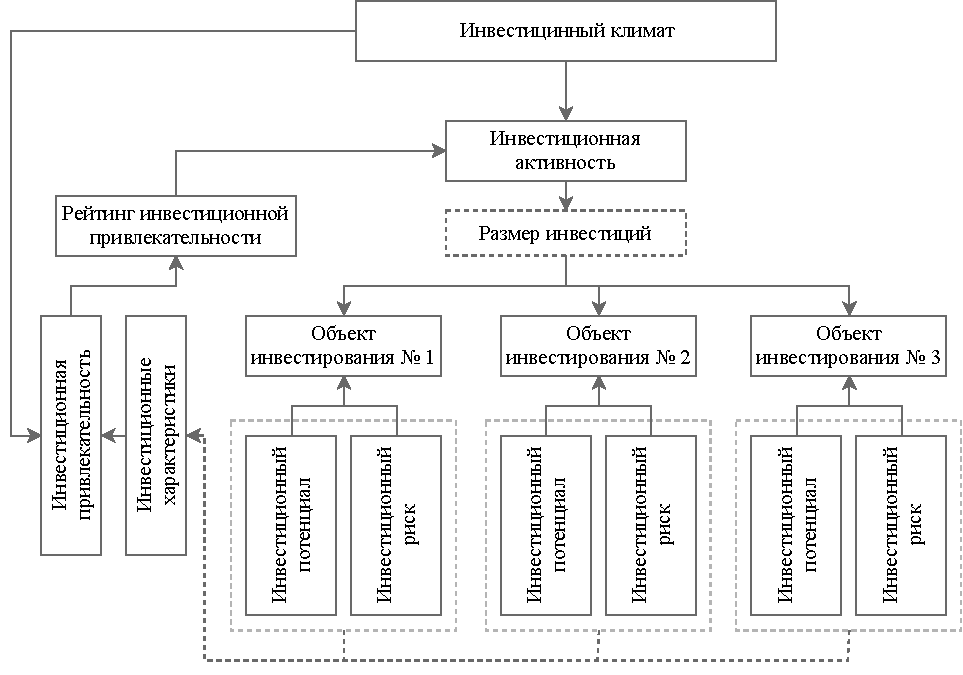
\includegraphics[width=1\linewidth]{invest}
	\caption{Взаимосвязь между инвестиционным климатом, инвестиционной активностью и инвестиционной привлекательностью}
	\label{fig:invest}
\end{figure}

Под инвестиционной активностью понимается динамика размера, структуры инвестиций, а также эффективность их использования.
Она напрямую зависит от рейтингов объектов инвестирования, публикуемых рейтинговыми агентствами и консалтинговыми компаниями.
В настоящее время рассчитываются рейтинги стран, субъектов федерации, городов и организаций.
Ключевое влияние на рейтинг оказывает инвестиционная привлекательность.
Она выражается в наборе качественных характеристик, делающих потенциальный объект  инвестирования безопасным и выгодным вложением для инвесторов.
Рейтинг может быть представлен с помощью индекса, на основе которого сравниваются объекты со схожими качественными характеристиками.

Степень инвестиционной привлекательности объекта зависит от инвестиционного потенциала и инвестиционного риска.
Она определяется совокупностью имеющихся объективных показателей и предпосылок для осуществления инвестиций (инвестиционный потенциал), а также вероятностью возникновения непредвиденных финансовых потерь в условиях неопределенности вложения капитала за счет изменения макроэкономической ситуации (инвестиционный риск).
Степень инвестиционной привлекательности отражается на размере инвестиций в различные объекты.

Российские исследователи выделяют следующие факторы, оказывающие влияние на инвестиционный климат:
\begin{itemize}
	\setlength\itemsep{0pt}
	\item политическая стабильность;
	\item нормативно-законодательная база и скорость ее изменения;
	\item состояние внутреннего рынка страны и ее финансовой системы;
	\item размер налогового бремени;
	\item платежеспособный спрос населения;
	\item квалификация персонала;
	\item стоимость ресурсов (сырьевых, трудовых, финансовых);
	\item информационное обеспечение;
	\item задолженность по внешним обязательствам перед международными экономическими и финансовыми организациями.
\end{itemize}

Согласно существующим критериям Россия в настоящее время относится к государствам со средним уровнем достигнутого экономического развития  и умеренными инвестиционными рисками.

Привлекательность вложения в страну финансовых средств определяется индексами деловой активности фондового рынка: в США --- DowJones и NASDAQ, в Европе --- EuroCtoxx 50,  в том числе FTSE (Лондон), XETRA DAX (Франкфурт-на-Майне), CAC-40 (Париж), SMI (Цюрих), AEX (Амстердам), MIBTel (Милан), IBEX (Мадрид), в Японии --- Nikke1-225, в Китае --- HANGSENQ, в России --- ММВБ-РТС и др.

Решение об инвестировании принимается после оценки инвестиционного климата страны и отдельного региона, в который планируется осуществить вложения.
В настоящее время разработаны и применяются следующие методики оценки инвестиционного климата:

1) универсальная методика оценки инвестиционного климата включает в себя максимальное количество экономических характеристик, показателей торговли, характеристик политического климата и законодательства.
Такая информационная база позволяет провести корректную оценку ситуации в стране на текущий момент и сделать прогноз относительно ее развития;

2) методика сравнительного анализа инвестиционного климата используется в государствах с переходной экономикой.
Ее основу составляют специализированные методики, позволяющие сделать акцент на темпах и перспективах реформ.
Информационной основой анализа являются данные опроса экспертов, представляющих крупные банки развитых стран.
Кроме этого, методика учитывает статистическую информацию о состоянии того или иного фактора развития экономики;

3) методика бальной оценки.
Она позволяет провести количественное сопоставление основных характеристик инвестиционного климата стран и определить показатели, которые учитывают величины всех составляющих и служат критерием ранжирования стран по их инвестиционной привлекательности.

Оценить инвестиционный климат России непросто.
Основная проблема, которая возникает при проведении оценки --- это наличие большой территории с различными климатическими условиями, природными ресурсами и другими факторами.
Поэтому чаще всего оценивают инвестиционный климат отдельных регионов, а не страны в целом.

В России существует большая дифференциация между регионами: существуют регионы, которые живут за счет субсидий из федерального бюджета, и регионы-доноры.

Ключевую роль на российском рынке оценки инвестиционного климата регионов занимает рейтинговое агентство <<Эксперт РА>>.
В качестве информационной базы агентство использует ежегодно собираемые по типовой методике данные Федеральной службы государственной статистики РФ, Министерства финансов РФ, министерства экономического развития РФ, Центрального банка РФ, Федеральной налоговой службы, Министерства внутренних дел РФ, а также базы новостных лент российских информационных агентств и собственные базы данных.
При оценке законодательного риска используется справочная правовая система <<КонсультантПлюс>>.
Для оценки распространения сотовой связи и интернета используются данные компании iKS-Consulting, результаты федеральных и региональных выборов публикуются на интернет-сайтах Центризбиркома РФ и избирательных комиссий субъектов Федерации.
При составлении рейтинга также используется информация по законодательству, стратегиям и программам регионального развития, представленная на сайтах регионов, а также предоставленная агентству администрациями отдельных субъектов Федерации по собственной инициативе \cite[с. 57--62]{borisova}.

Инвестиционная привлекательность в рейтинге оценивается по двум параметрам: инвестиционному потенциалу и инвестиционному риску.

Потенциал показывает, какую долю регион занимает на общероссийском рынке, риск --- какими могут быть для инвестора масштабы тех или иных проблем в регионе.
Суммарный потенциал состоит из девяти частных: трудового, финансового, производственного, потребительского, институционального, инфраструктурного, природно-ресурсного, туристического и инновационного.

Интегральный риск состоит из шести частных: финансового, социального, управленческого, экономического, экологического и криминального.
Вклад каждого частного риска или потенциала в итоговый индикатор оценивается на основе анкетирования представителей экспертного, инвестиционного и банковского сообществ.

Рейтинг инвестиционной привлекательности регионов России 2017 года впервые за долгое время демонстрирует снижение интегрального инвестриска и всех его частных составляющих. Самая острая фаза кризиса пройдена и в показателях 2016-го, это отразилось в сокращении интегрального инвестиционного риска на 3,1\% относительно уровня 2015 года. Наибольшее снижение у финансового риска (-4,8\%), а наименьшее – у управленческого (-1,2\%).

Произошедшее в кризис размывание понятного набора рычагов воздействия на экономический рост требует от региональных властей усложнения управленческого инструментария. Волна отставок и назначений в губернаторском корпусе свидетельствует, что ответ на новые вызовы оказались способны найти далеко не все руководители территорий. Из анализа рейтинга необходимость перемен в составе региональных команд вытекает вполне четко: почти в 2/3 субъектов Федерации, где произошла смена губернатора, показатели социальных, финансовых и экономических рисков по итогам 2014–2016 годов были заметно хуже средних.

Благодаря агломерационному эффекту первыми частичное выправление ситуации почувствовали крупнейшие экономические центры страны. В нынешнем рейтинге 12 из 17 регионов, в состав которых входят города-миллионники, включая пристоличные области (Московская и Ленинградская), улучшили свое положение по показателю интегрального риска. Так, Петербург прибавил 3 позиции, Новосибирская область – 6, Волгоградская – целых 10, а Московская – 4, выйдя в лидеры списка.

Рейтинг показывает, что многим регионам предстоит пережить смену экономической парадигмы. Если до кризиса роль тех или иных региональных драйверов была очевидной для конкретных территорий, то сейчас картина социально-экономического развития в региональном преломлении стала расфокусированной. Так, Ростовская область, считающаяся по преимуществу аграрной, в нынешнем рейтинге поднялась на 3 позиции в первую очередь за счет машиностроительных предприятий, равно как и традиционно индустриальные Иркутская и Ульяновская области – плюс 4 и 3 позиции соответственно.

Нынешний рейтинг отражает постепенное прекращение живительного воздействия инъекций «нефтяной иглы». Заметно сдали позиции Ханты-Мансийский автономный округ – Югра (минус 8 мест по риску) и Омская область (минус 5).

Влияние агропромышленного комплекса после очевидного эффекта, вызванного девальвацией, ослабло. Из-за неблагоприятной мировой ценовой конъюнктуры, способствовавшей снижению экспорта, в 2016 году показатели ряда мощных зерновых регионов страны просели с точки зрения инвестпривлекательности. Это стало одной из причин перемещения Краснодарского края с 1-й строчки на 4-ю по интегральному инвестриску и Ставрополья с 16-й позиции на 24-ю. Схожую динамику в рейтинге показал и ряд областей Центрального Черноземья: Тамбовская (5-е место против 2-го годом ранее), Курская (10-е и 6-е) и Орловская (62-е и 58-е). Лучше в рейтинге показали себя регионы, где в последнее время идет активное наращивание производства и переработки говядины (вложения в производство свинины и мяса птицы сыграли свою роль в прошлые годы), – это прежде всего Белгородская (переход с 8-го места в прошлом рейтинге на 7-е в нынешнем) и Брянская (31-я и 36-я позиции соответственно) области. Тем не менее, потенциал развития АПК и его влияния на экономики территорий далек от исчерпания, в том числе и в связи с продолжающейся господдержкой сектора.

На выходе из кризиса заметно снизилось стимулирующее воздействие на региональные экономики федеральных программ. Наиболее показательны в этом отношении Крым и Севастополь – в нынешнем рейтинге эти два региона переместились вниз на 5 и 6 позиций соответственно из-за очевидных сбоев в управлении, выразившихся в неспособности осваивать бюджетные средства и вовлекать местный бизнес в реализацию крупных проектов. Снижение эффекта от бюджетных вливаний на экономику продемонстрировала и Амурская область (падение на 16 позиций по интегральному показателю риска) из-за паузы в строительстве следующих очередей космодрома Восточный.

Предпосылки для роста региональных экономик создало проведенное государством оздоровление региональных бюджетов. После долгих лет неизменного роста началось сокращение долговой нагрузки на бюджеты субъектов РФ, которое сопровождалось и оздоровлением структуры долга: за январь – сентябрь 2017 года портфель банковских кредитов региональным бюджетам сократился на 33\%, почти половина от этого сокращения – заслуга займов из федерального бюджета. При осмысленном выборе приоритетов и грамотной экономической политике средства, не потраченные на погашение высоких процентов по коммерческим кредитам, можно будет пустить на развитие \cite{expertra}.












\subsection{Принципы оценки эффективности инвестиционного проекта}

Процессу инвестирования как правило предшествует разработка инвестиционного проекта. Инвестпроект позволяет оценить потребность в инвестициях, их распределение во времени, спрогнозировать доходность предполагаемых инвестиций, оценить риски инвестирования. На основании данной информации принимается решение об инвестировании \cite[с. 82]{borisova}.

Федеральный закон <<Об инвестиционной деятельности в РФ, осуществляемой в форме капитальных вложений>> \cite{39-fz} дает следующее определение.
\begin{quote}
	Под инвестиционным проектом понимается обоснование экономической целесообразности, объема и сроков осуществления капитальных вложений, в том числе необходимая проектно-сметная документация, разработанная в соответствии с законодательством РФ и утвержденными в установленном порядке стандартами (нормами и правилами), а также описание практических действий по осуществлению инвестиций (бизнес-план).
\end{quote}


В данном случае речь идет о проектах, направленных на создание реальных физических объектов (заводов, жилых домов и т.д.). Если же организации необходимо купить пакет акций другой компании, такая сделка также считается инвестпроектом.

Далее рассмотрим классификацию инвестиционных проектов по различным признакам.

По отношению друг к другу инвестпроекты бывают:
\begin{enumerate}
	\setlength\itemsep{0pt}
	\item [---] независимые (допускают одновременное и раздельное осуществление; характеристики реализации не влияют друг на друга);
	\item [---] альтернативные (не допускают одновременной реализации);
	\item [---] взаимодополняющие (реализация может происходить только совместно).
\end{enumerate}

По срокам реализации:
\begin{enumerate}
	\setlength\itemsep{0pt}
	\item [---] краткосрочные --- до трех лет;
	\item [---] среднесрочные --- от трех до пяти лет;
	\item [---] долгосрочные --- свыше пяти лет.
\end{enumerate}

По масштабам (величине капитальных вложений):
\begin{enumerate}
	\setlength\itemsep{0pt}
	\item [---] малые;
	\item [---] средние;
	\item [---] крупные;
	\item [---] мегапроекты.
\end{enumerate}

В России параметры для отнесения проектов к этим категориям не установлены.

По направленности:
\begin{enumerate}
	\setlength\itemsep{0pt}
	\item [---] коммерческие (главная цель --- получение прибыли);
	\item [---] социальные (цель --- решение определенных социальных проблем --- развитие спорта, образования, медицины и т.д.);
	\item [---] экологические (целью является решение экологических проблем, улучшение экологии и т.д.).
\end{enumerate}

Эта классификация носит чисто условный характер. Большинство коммерческих проектов приносит также социальную выгоду.


В зависимости от величины риска:
\begin{enumerate}
	\setlength\itemsep{0pt}
	\item [---] надежные (безрисковые) проекты --- вероятность получения гарантированных результатов высокая;
	\item [---] рисковые проекты --- характеризуются высокой степенью неопределенности затрат и результатов.
\end{enumerate}

Любой инвестиционный проект состоит из трех основных элементов (рисунок \ref{fig:element}).

\begin{figure}[!ht]
	\centering
	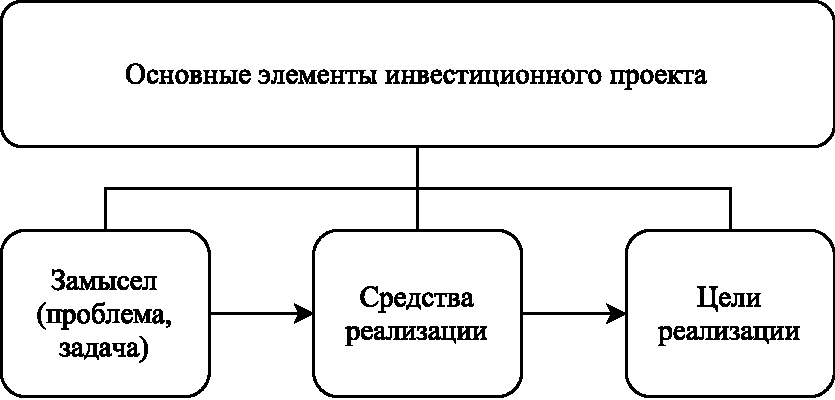
\includegraphics[width=0.7\linewidth]{element}
	\caption{Основные элементы инвестиционного проекта}
	\label{fig:element}
\end{figure}

Жизненным циклом инвестиционного проекта считается временной интервал между моментом появления и окончания реализации проекта. Окончанием обычно является ввод в действие объектов, достижение проектом заданных результатов, прекращение финансирования проекта, вывод проекта из эксплуатации.

На рисунке \ref{fig:prcycle} показаны три фазы жизненного цикла инвестпроекта: предынвестиционная, инвестиционная и эксплуатационная.

\begin{figure}[!hb]
	\centering
	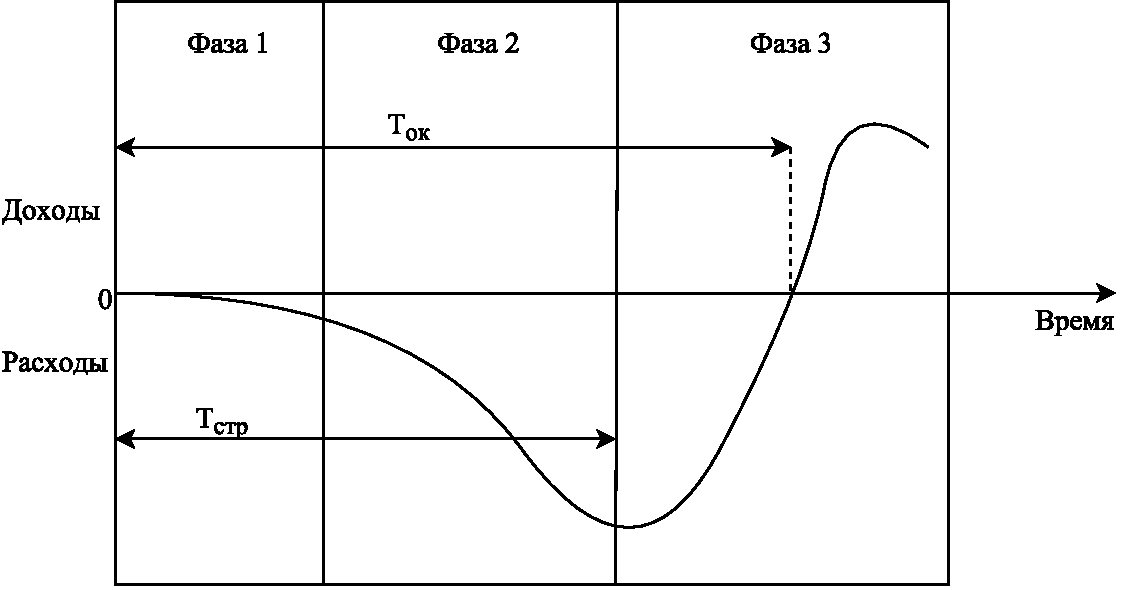
\includegraphics[width=0.85\linewidth]{prcycle}
	\caption{Жизненный цикл инвестиционного проекта}
	\label{fig:prcycle}
\end{figure}

Фаза 1 --- предынвестиционная, подготовительная стадия, предшествует основному объему инвестирования. Сюда входит юридическое оформление инвестпроекта, поиск источников финансирования и др.

Фаза 2 --- инвестиционная, включает инвестирование и осуществление проекта.

Фаза 3 --- эксплуатационная (производственная), начинается после ввода объекта в эксплуатацию и является самой продолжительной.

Наиболее значимыми качественными параметрами инвестпроекта являются срок строительства ($\text{Т}_{\text{стр}}$) и срок окупаемости ($\text{Т}_{\text{ок}}$).

Срок строительства связан с рациональным использованием ресурсов в период 1 и 2 фазы. Срок окупаемости же зависит от всех трех стадий инвестпроекта, но такие параметры проекта, как качество и эффективность доказываются на эксплуатационной стадии \cite[с. 162--166]{sergeev}

\subsection{Основные мероприятия, направленные на снижение инвестиционных рисков в проектах}

Управление рисками является составной частью управления коммерческой организацией в целом, поэтому в ней должно быть и функциональное подразделение, отвечающее за этот участок работы.
Обычно это финансовый менеджер.

При управлении рисками следует соблюдать следующие правила, выработанные наукой и практикой:
\begin{enumerate}
	\setlength\itemsep{0pt}
	\item не рисковать больше, чем может позволить собственный капитал;
	\item надо думать о последствиях риска;
	\item нельзя рисковать многим ради одного;
	\item нельзя класть все яйца в одну корзину;
	\item положительное решение принимается лишь при отсутствии сомнения, в противном случае принимается отрицательное решение;
	\item нельзя думать, что существует только одно решение. Возможно есть и другие.
\end{enumerate}

Реализация первого правила означает, что прежде, чем принять решение о рисковом вложении капитала, надо определить максимально возможный объем убытка по данному риску, соотнести его с объемом вкладываемого капитала, сопоставить его со всеми собственными финансовыми ресурсами и определить, не приведет ли потеря этого капитала к банкротству инвестора.

Соотношение максимально возможного объема убытка и объема собственных финансовых ресурсов инвестора представляет собой степень риска, ведущего к банкротству.
Ее измеряют с помощью коэффициента риска \cite[241]{sergeev}
\[ \text{К}_\text{р} = \frac{\text{У}}{\text{С}}, \]\\
где У --- максимально возможная сумма убытка; С --- объем собственных финансовых ресурсов с учетом точно известных поступлений средств.

По мнению И. Т. Балабанова, оптимальный коэффициент риска составляет 0,3, а коэффициент риска, ведущий к банкротству инвестора --- 0,7 и более.

При управлении инвестиционными рисками используют ряд приемов, которые состоят, в основном, из средств разрешения рисков и приемов снижения степени риска.

Средствами разрешения рисков являются их избежание, удержание, передача, снижение степени риска.

Избежание риска означает простое уклонение от мероприятия, связанного с риском.
Однако избежание риска для инвестора чаще является отказом от прибыли.

Удержание риска --- оставление риска за инвестором, т.е. на его ответственности.

Передача риска означает, что инвестор передает ответственность за риск кому-то другому, например страховой компании.
В данном случае передача риска происходит путем его страхования.

Снижение степени риска — сокращение вероятности и объема потерь.

Для снижения степени риска используют различные приемы, из которых наиболее распространенными являются: диверсификация, приобретение достоверной и полной информации, лимитирование, самострахование, страхование.

Наиболее известным и распространенным из этих приемов является диверсификация, реализующая правило «нельзя класть яйца в одну корзину».
Под диверсификацией в широком смысле понимается сознательный подбор комбинаций инвестиционных проектов, когда достигается не просто их разнообразие, а определенная взаимозависимость динамики доходов и приемлемый уровень рискованности.
Диверсификации могут быть подвергну ты как реальные, так и портфельные инвестиции.

Диверсификация реальных инвестиций в основном направлена на создание диверсифицированного производства, т.е. на расширение номенклатуры и ассортимента выпускаемой продукции не только основного производства, но и продукции и услуг, не свойственных данному предприятию.
В этом случае риск банкротства предприятия существенно снижается  \cite[242]{sergeev}.

Диверсификация портфельных инвестиций на предприятии должна быть направлена на создание такого портфеля ценных бумаг, который был бы оптимальным как по уровню доходности, так и по степени риска.

Исходя из этого можно сделать вывод, что диверсификация как реальных, так и портфельных инвестиций является одним из действенных направлений по снижению инвестиционных рисков, но из этого не следует, что во всех случаях необходимо прибегать к диверсификации производства.
Если предприятие является узкоспециализированным, а его продукция --- конкурентоспособной как на данном этапе, так и в перспективе, то вряд ли целесообразно прибегать к диверсификации производства.

Важным фактором для снижения степени инвестиционных рисков являются достоверность и полнота информации, на основе которых принимаются инвестиционные решения.
Вся эта информация, в зависимости от источника ее получения, может быть классифицирована следующим образом: 
\begin{itemize}
\setlength\itemsep{0pt}
\item информация, полученная из официальных, открыто публикуемых источников (статистические сборники, газеты и журналы, экономическая и социальная политика государства и др.); 
\item  информация, полученная по закрытым каналам; 
\item  информация, полученная на основе обработки и анализа статистической и иной информации.
\end{itemize}

Полная и достоверная информация --- товар особого рода, за который надо платить, но эти расходы окупаются в результате получения существенной выгоды от вложения инвестиций.

Лимитирование --- установление предприятием предельно допустимой суммы средств на выполнение определенных операций, в случае невозврата которой это несущественно отразится на финансовом состоянии предприятия.
Оно является важным приемом снижения степени риска и применяется банками при выдаче ссуд, а промышленными предприятиями -- при продаже товаров в кредит, предоставлении займов, определении сумм вложения капитала, а также в других случаях.

Страхование и самострахование являются важными приемами по снижению степени риска.
Страховые компании получили довольно широкое распространение во многих странах мира, но особенно --- в странах с развитой рыночной экономикой. Идет процесс становления страхового дела и в России.

Страхование --- отношения по защите имущественных интересов хозяйствующих субъектов при наступлении определенных событий (страховых случаев) за счет денежных фондов, формируемых из уплачиваемых ими страховых взносов (страховых премий).
Другими словами, сущность страхования заключается в распределении ущерба между участниками страхования.
Страхование --- это платная функция, независимо от того, наступит или не наступит случай потери имущества, поэтому некоторые хозяйствующие субъекты, если это не обязательное страхование, для снижения степени риска применяют самострахование.

Самострахование означает, что предприниматель предпочитает подстраховаться сам, чем покупать страховку в страховой компании.
Тем самым он экономит затраты по страхованию.
Самострахование представляет собой децентрализованную форму создания натуральных и денежных страховых (резервных) фондов непосредственно в хозяйствующем субъекте, особенно в тех, чья деятельность подвержена риску.

Мы рассмотрели некоторые приемы снижения инвестиционного риска, которые известны и изложены в отечественной и зарубежной литературе.
Но самый верный прием снижения степени риска --- компетентное управление предприятием (организацией), начиная с момента создания и на всех последующих эта пах его функционирования.
При этом никогда не следует забывать, что могут произойти негативные явления, не зависящие от управленческого персонала, но и к ним предприятие должно быть в определенной степени готово.
Во всем этом и заключает ся смысл искусства управления \cite[243--244]{sergeev}.